\documentclass{standalone}
\usepackage{tikz}
\usetikzlibrary[arrows,positioning,matrix]

\begin{document}
\begin{tikzpicture}
  \node[draw=none] (example) {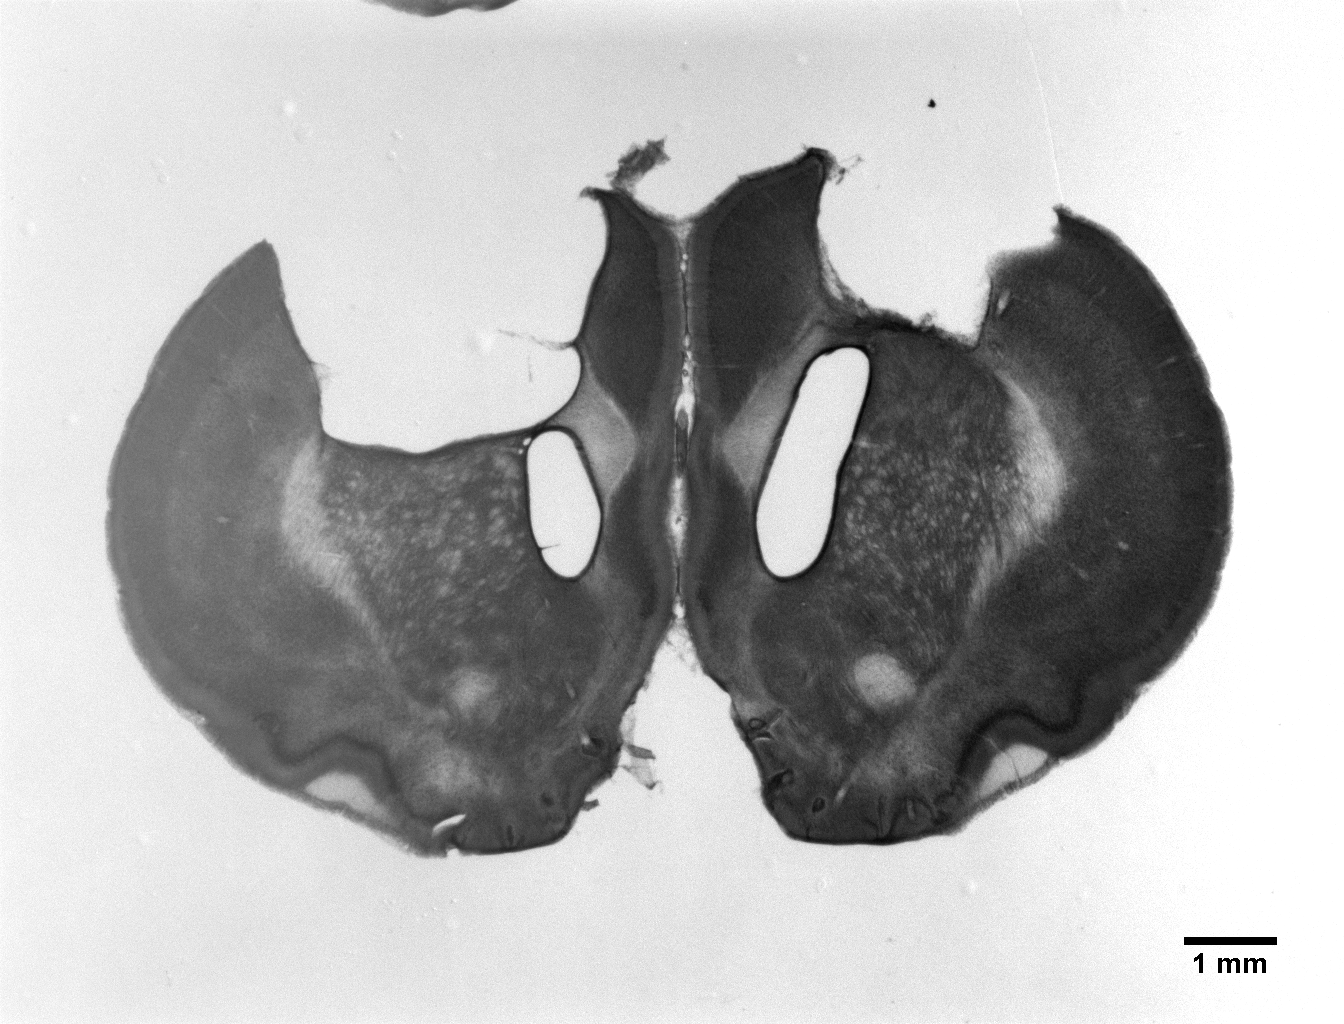
\includegraphics[width=0.33\textwidth]{elements/extendedlesionB_viewplate_bregma2mm-slice32}};
  \node[draw=none,above left=1.5mm and -4mm of example] {A};
  
  \node[draw=none,right=1mm of example] (schematic) {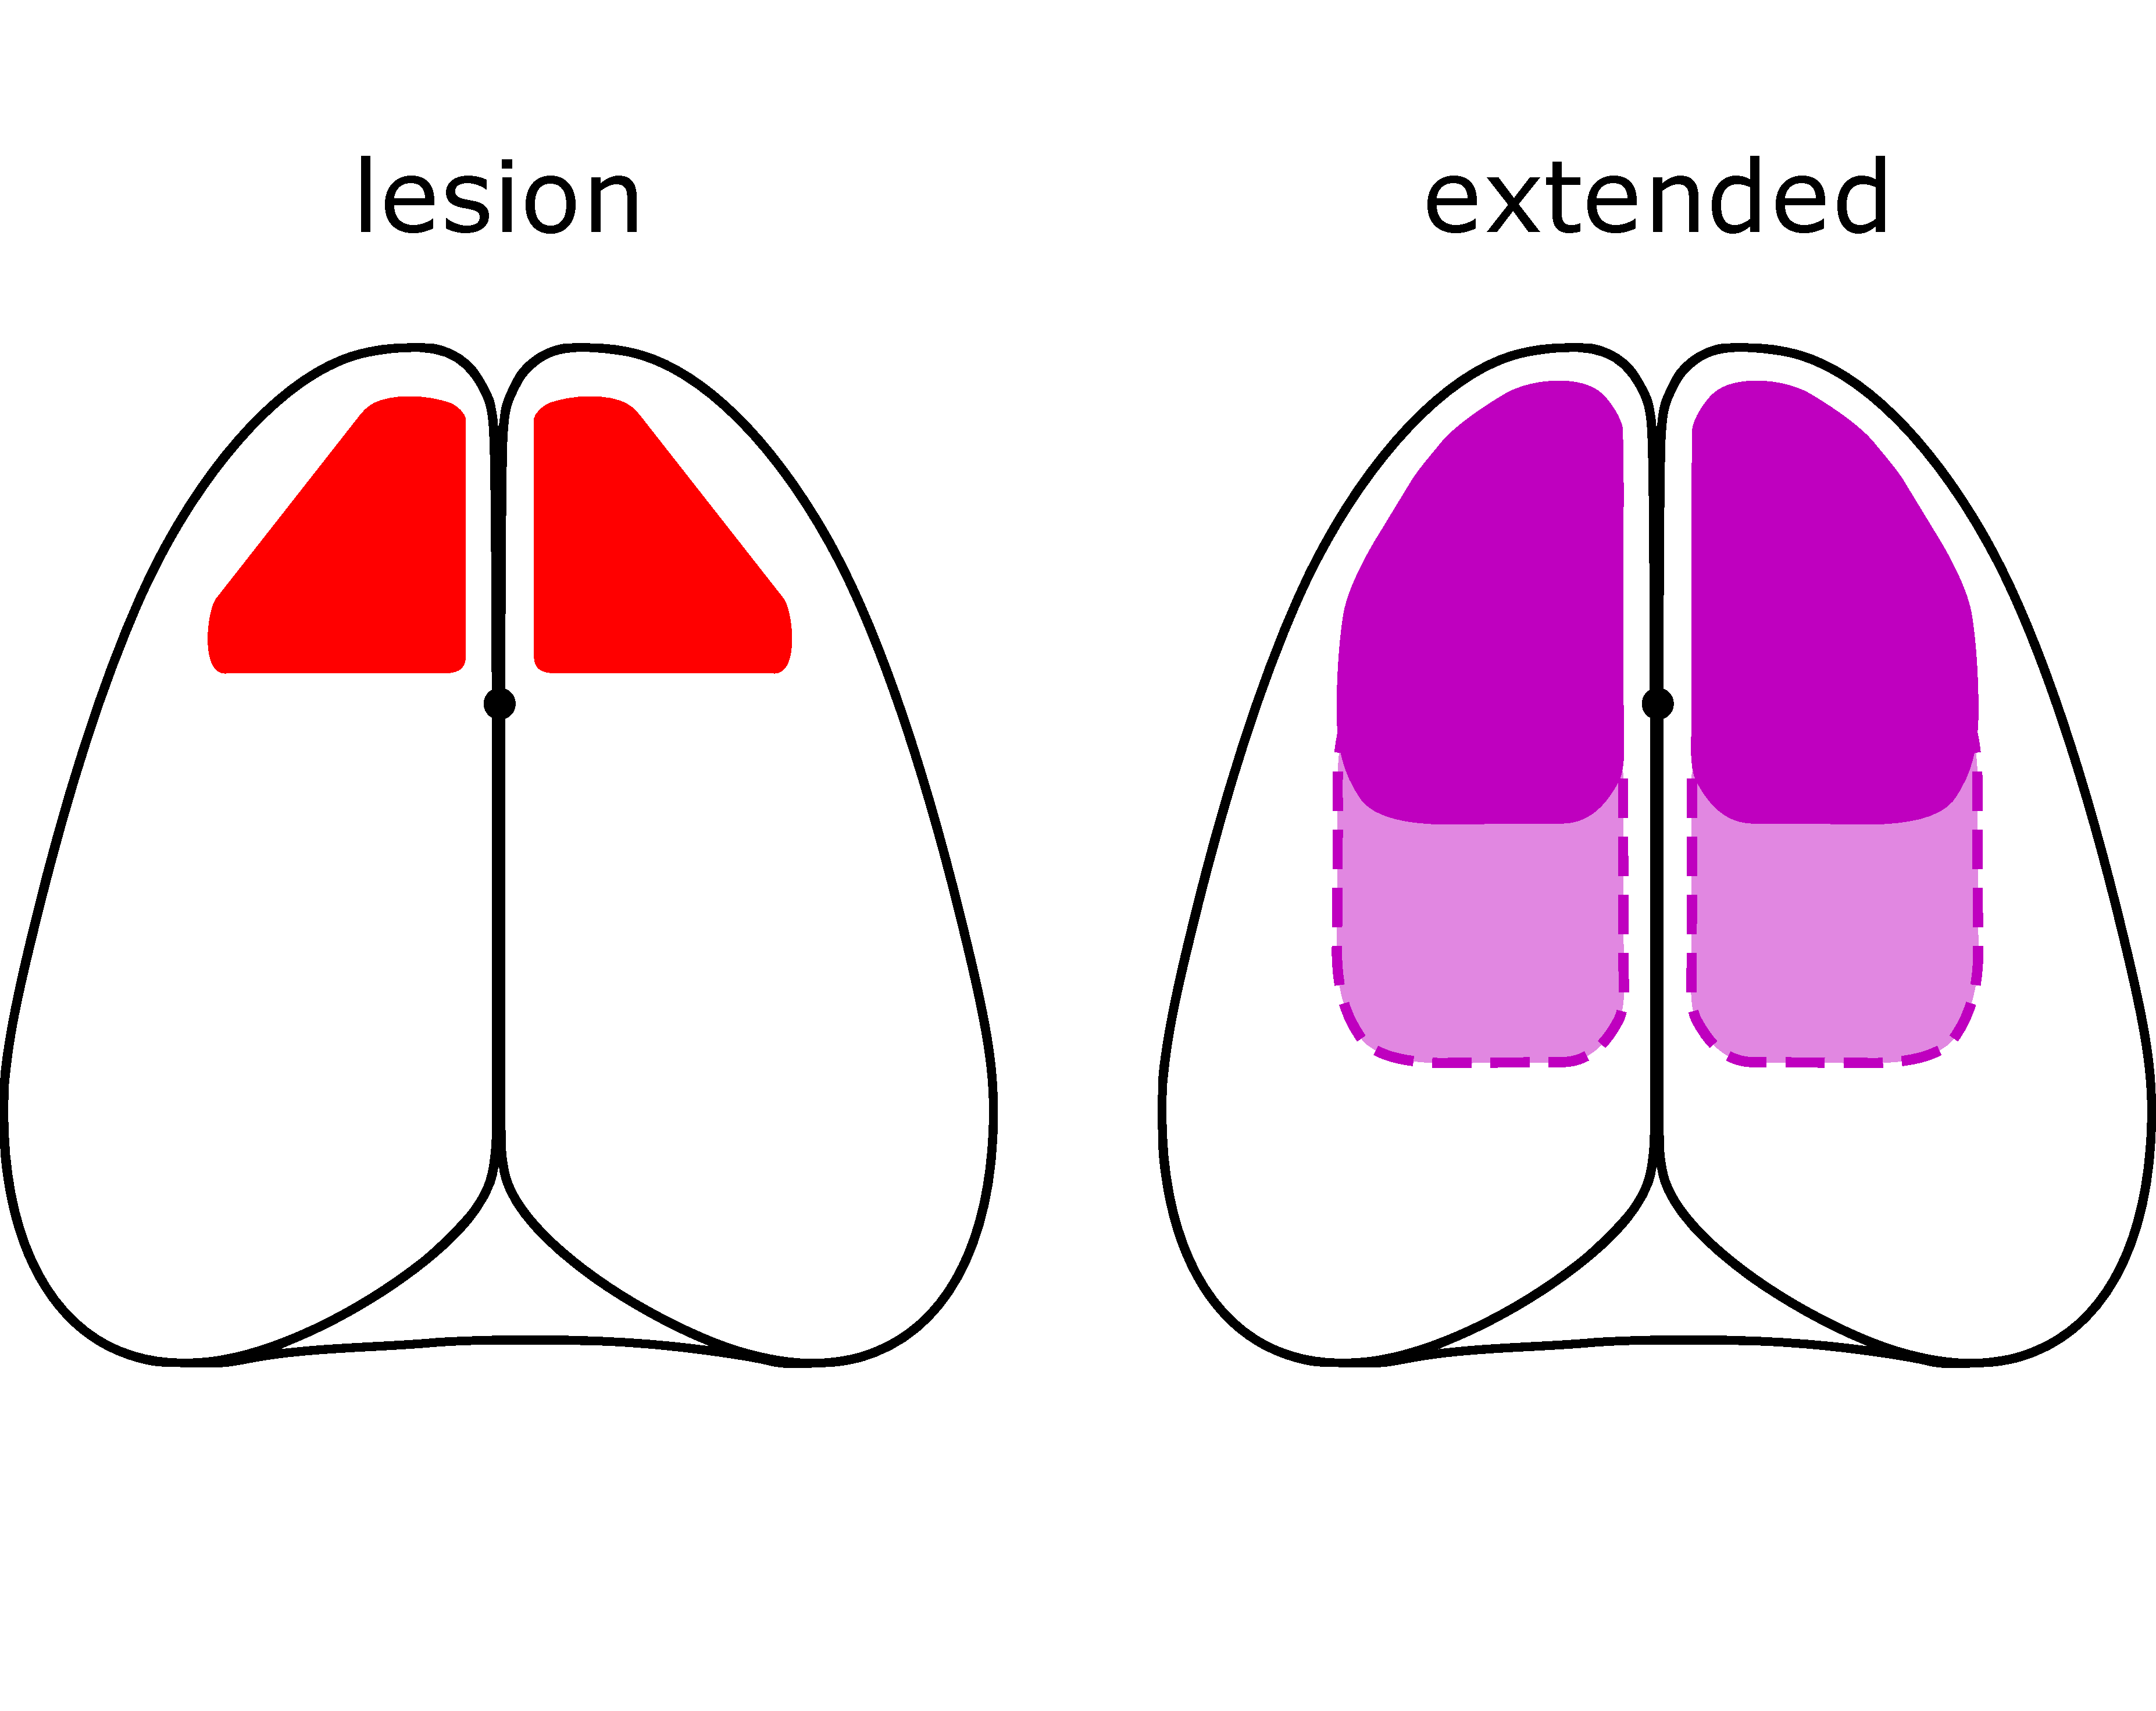
\includegraphics[width=0.33\textwidth]{elements/extendedlesions}};
  \node[draw=none,above left=0.6mm and -4mm of schematic] {B};
  
  \node[draw=none,right=1mm of schematic] (learning) {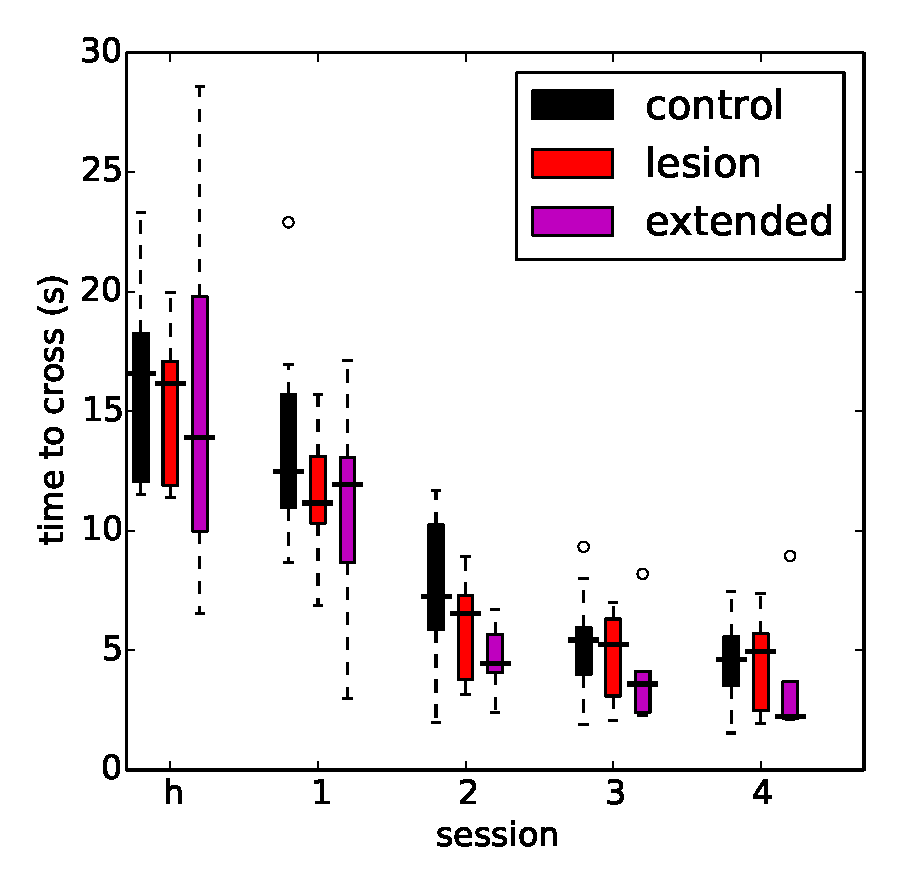
\includegraphics[width=0.33\textwidth]{elements/timetocross_extended}};
  \node[draw=none,above left=-3mm and -4mm of learning] {C};
  
  \node[draw=none,below=7.5mm of example] (slipanalysis) {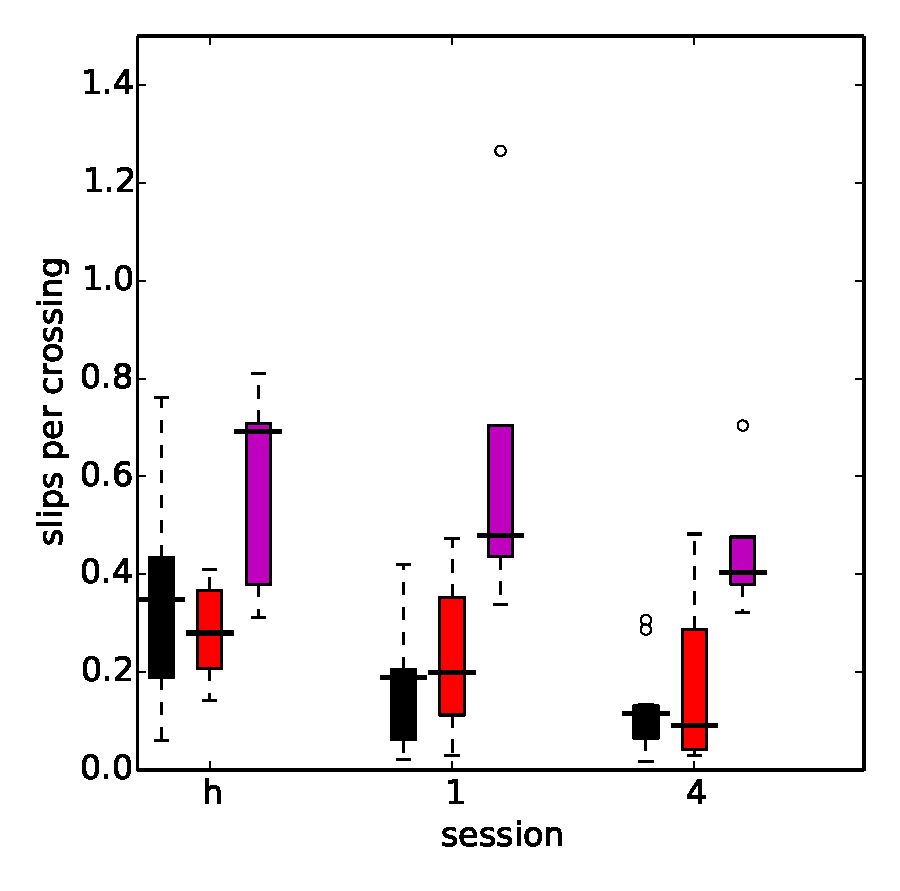
\includegraphics[width=0.33\textwidth]{elements/slipanalysis}};
  \node[draw=none,above=-2mm of slipanalysis] {paw slips};
  \node[draw=none,above left=-3mm and -4mm of slipanalysis] {D};

  \node[draw=none,right=1mm of slipanalysis] (slipforelimb) {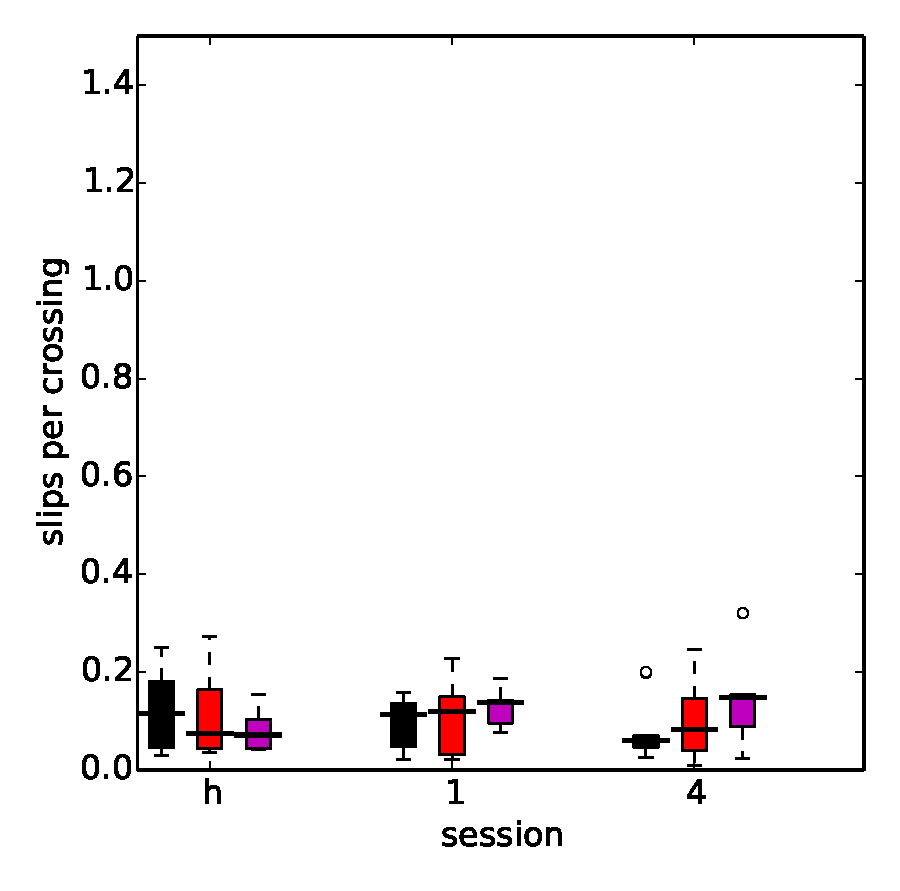
\includegraphics[width=0.33\textwidth]{elements/slipanalysis_forelimb}};
  \node[draw=none,above=-2mm of slipforelimb] {forelimbs};
  \node[draw=none,above left=-3mm and -4mm of slipforelimb] {E};
  
  \node[draw=none,right=1mm of slipforelimb] (sliphindlimb) {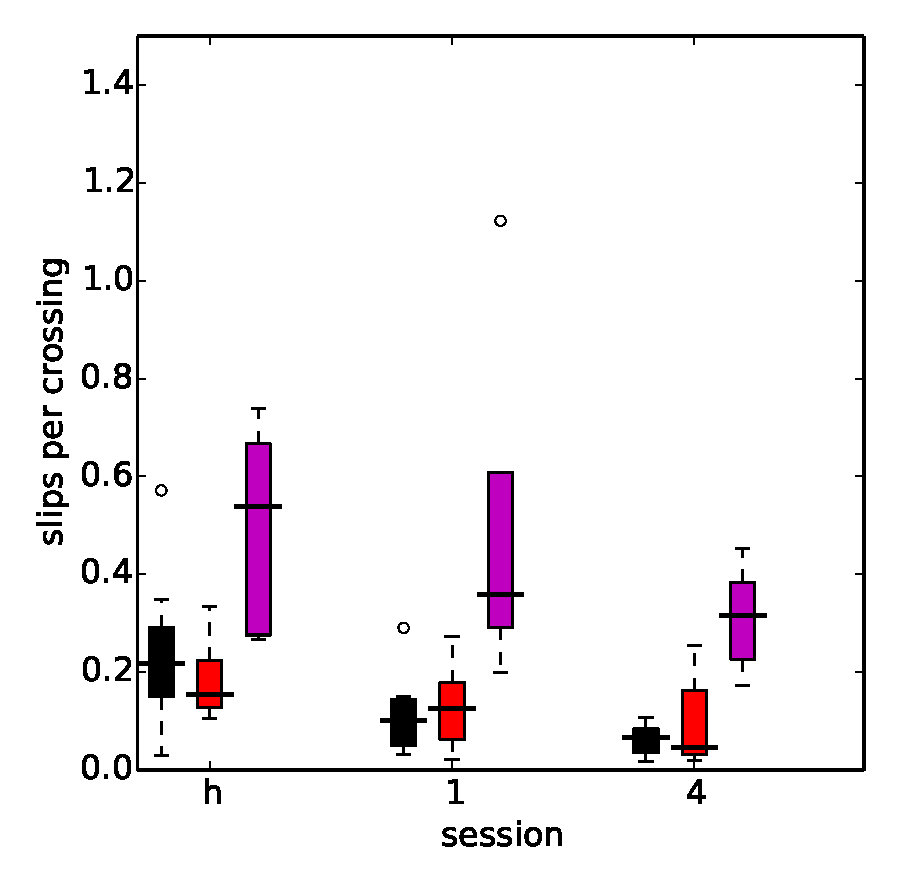
\includegraphics[width=0.33\textwidth]{elements/slipanalysis_hindlimb}};
  \node[draw=none,above=-2mm of sliphindlimb] {hindlimbs};
  \node[draw=none,above left=-3mm and -4mm of sliphindlimb] {F};
\end{tikzpicture}
\end{document}